% Options for packages loaded elsewhere
\PassOptionsToPackage{unicode}{hyperref}
\PassOptionsToPackage{hyphens}{url}
\PassOptionsToPackage{dvipsnames,svgnames,x11names}{xcolor}
%
\documentclass[
  ignorenonframetext,
]{beamer}
\usepackage{pgfpages}
\setbeamertemplate{caption}[numbered]
\setbeamertemplate{caption label separator}{: }
\setbeamercolor{caption name}{fg=normal text.fg}
\beamertemplatenavigationsymbolsempty
% Prevent slide breaks in the middle of a paragraph
\widowpenalties 1 10000
\raggedbottom
\setbeamertemplate{part page}{
  \centering
  \begin{beamercolorbox}[sep=16pt,center]{part title}
    \usebeamerfont{part title}\insertpart\par
  \end{beamercolorbox}
}
\setbeamertemplate{section page}{
  \centering
  \begin{beamercolorbox}[sep=12pt,center]{part title}
    \usebeamerfont{section title}\insertsection\par
  \end{beamercolorbox}
}
\setbeamertemplate{subsection page}{
  \centering
  \begin{beamercolorbox}[sep=8pt,center]{part title}
    \usebeamerfont{subsection title}\insertsubsection\par
  \end{beamercolorbox}
}
\AtBeginPart{
  \frame{\partpage}
}
\AtBeginSection{
  \ifbibliography
  \else
    \frame{\sectionpage}
  \fi
}
\AtBeginSubsection{
  \frame{\subsectionpage}
}
\usepackage{amsmath,amssymb}
\usepackage{lmodern}
\usepackage{iftex}
\ifPDFTeX
  \usepackage[T1]{fontenc}
  \usepackage[utf8]{inputenc}
  \usepackage{textcomp} % provide euro and other symbols
\else % if luatex or xetex
  \usepackage{unicode-math}
  \defaultfontfeatures{Scale=MatchLowercase}
  \defaultfontfeatures[\rmfamily]{Ligatures=TeX,Scale=1}
\fi
% Use upquote if available, for straight quotes in verbatim environments
\IfFileExists{upquote.sty}{\usepackage{upquote}}{}
\IfFileExists{microtype.sty}{% use microtype if available
  \usepackage[]{microtype}
  \UseMicrotypeSet[protrusion]{basicmath} % disable protrusion for tt fonts
}{}
\makeatletter
\@ifundefined{KOMAClassName}{% if non-KOMA class
  \IfFileExists{parskip.sty}{%
    \usepackage{parskip}
  }{% else
    \setlength{\parindent}{0pt}
    \setlength{\parskip}{6pt plus 2pt minus 1pt}}
}{% if KOMA class
  \KOMAoptions{parskip=half}}
\makeatother
\usepackage{xcolor}
\newif\ifbibliography
\setlength{\emergencystretch}{3em} % prevent overfull lines
\providecommand{\tightlist}{%
  \setlength{\itemsep}{0pt}\setlength{\parskip}{0pt}}
\setcounter{secnumdepth}{-\maxdimen} % remove section numbering
\newlength{\cslhangindent}
\setlength{\cslhangindent}{1.5em}
\newlength{\csllabelwidth}
\setlength{\csllabelwidth}{3em}
\newlength{\cslentryspacingunit} % times entry-spacing
\setlength{\cslentryspacingunit}{\parskip}
\newenvironment{CSLReferences}[2] % #1 hanging-ident, #2 entry spacing
 {% don't indent paragraphs
  \setlength{\parindent}{0pt}
  % turn on hanging indent if param 1 is 1
  \ifodd #1
  \let\oldpar\par
  \def\par{\hangindent=\cslhangindent\oldpar}
  \fi
  % set entry spacing
  \setlength{\parskip}{#2\cslentryspacingunit}
 }%
 {}
\usepackage{calc}
\newcommand{\CSLBlock}[1]{#1\hfill\break}
\newcommand{\CSLLeftMargin}[1]{\parbox[t]{\csllabelwidth}{#1}}
\newcommand{\CSLRightInline}[1]{\parbox[t]{\linewidth - \csllabelwidth}{#1}\break}
\newcommand{\CSLIndent}[1]{\hspace{\cslhangindent}#1}
\setbeamertemplate{footline}{\begin{beamercolorbox}{section in head/foot}

\includegraphics[height=.5cm]{../Images/egap-logo.png} \hfill
\insertframenumber/\inserttotalframenumber \end{beamercolorbox}}

\ifLuaTeX
  \usepackage{selnolig}  % disable illegal ligatures
\fi
\IfFileExists{bookmark.sty}{\usepackage{bookmark}}{\usepackage{hyperref}}
\IfFileExists{xurl.sty}{\usepackage{xurl}}{} % add URL line breaks if available
\urlstyle{same} % disable monospaced font for URLs
\hypersetup{
  pdftitle={Survey Experiments},
  pdfauthor={Jake Bowers, Nahomi Ichino and Maarten Voors},
  colorlinks=true,
  linkcolor={Maroon},
  filecolor={Maroon},
  citecolor={Blue},
  urlcolor={Blue},
  pdfcreator={LaTeX via pandoc}}

\title{Survey Experiments}
\author{Jake Bowers, Nahomi Ichino and Maarten Voors}
\date{09 June, 2022}

\begin{document}
\frame{\titlepage}

\begin{frame}[allowframebreaks]
  \tableofcontents[hideallsubsections]
\end{frame}
\hypertarget{overview-why-what-when-survey-experiments}{%
\section{Overview: Why, What, When Survey
Experiments}\label{overview-why-what-when-survey-experiments}}

\begin{frame}[allowframebreaks]{Key points for this lecture}
\protect\hypertarget{key-points-for-this-lecture}{}
\begin{itemize}
\item
  A survey experiment involves a randomized experiment within a survey.
  See
  \href{https://egap.org/resource/10-things-to-know-about-survey-experiments/}{10
  Things to Know About Survey Experiments}. See also Mutz
  (\protect\hyperlink{ref-mutz2011population}{2011}). See also
  \href{https://www.tessexperiments.org}{Time Sharing Experiments in the
  Social Sciences}.
\item
  Two types:

  \begin{itemize}
  \tightlist
  \item
    For \textbf{measuring} otherwise hard to measure concepts:
    ``Hostility toward female candidates'',``Anti-black prejudice'',
    ``Willingness to pay''
  \item
    For \textbf{causal inference} to learn about a theory (of attitudes,
    of behavior (when people are offered a behavioral outcome), beliefs,
    judgement).
  \end{itemize}
\item
  How?

  \begin{itemize}
  \tightlist
  \item
    All survey modes can have randomization of content to display to
    respondents.
  \item
    Randomization is much easier if you use a tablet or online or
    otherwise computer aided survey. (But you can do simple
    randomization with paper questionnares.)
  \end{itemize}
\item
  Why or When?

  \begin{itemize}
  \tightlist
  \item
    You want to learn about theories that explain attitudes, beliefs,
    behaviors of lots of people.
  \item
    A focus on individual people and what they say and can do in the
    context of a survey.
  \item
    Sometimes the \textbf{sample} of people contacted in a survey
    \textbf{represents} a population well. (Say, if the sample is
    random.)
  \item
    Survey experiments done online can be cheap.
  \item
    Computer aided survey experiments can allow large scale access to
    lab experiment-style research.
  \end{itemize}
\end{itemize}
\end{frame}

\hypertarget{example-treatments-for-causal-inference}{%
\section{Example Treatments for Causal
Inference}\label{example-treatments-for-causal-inference}}

\begin{frame}{Photos and Ballots}
\protect\hypertarget{photos-and-ballots}{}
\begin{figure}

{\centering 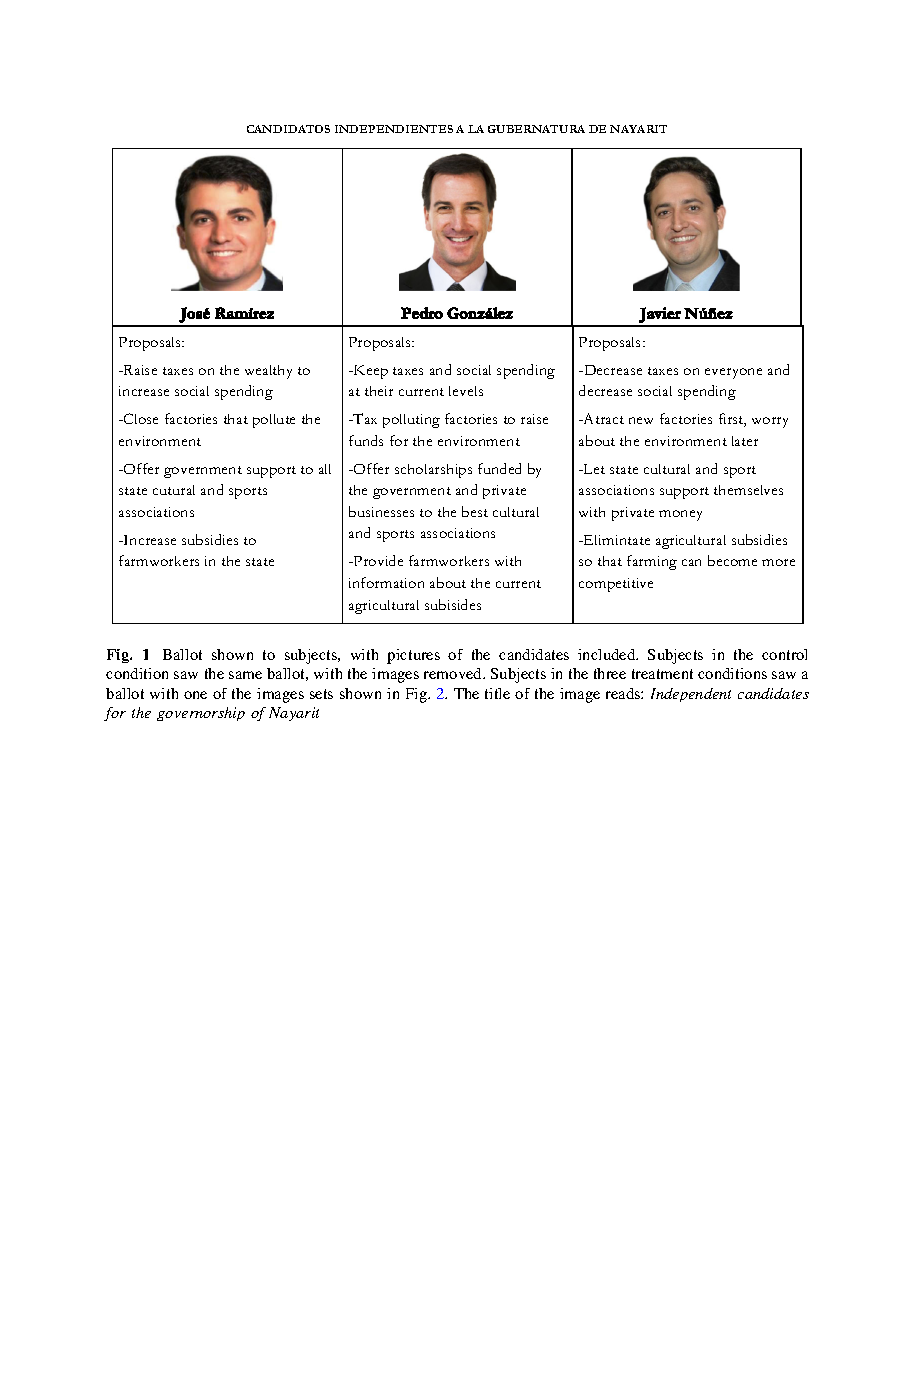
\includegraphics[width=0.7\linewidth]{./figs/survey-exp-aguilar-18_ballots} 

}

\end{figure}

Outcome: Candidate Choice (Aguiler et al 2018).
\end{frame}

\begin{frame}{Photos and Ballots}
\protect\hypertarget{photos-and-ballots-1}{}
\begin{figure}

{\centering 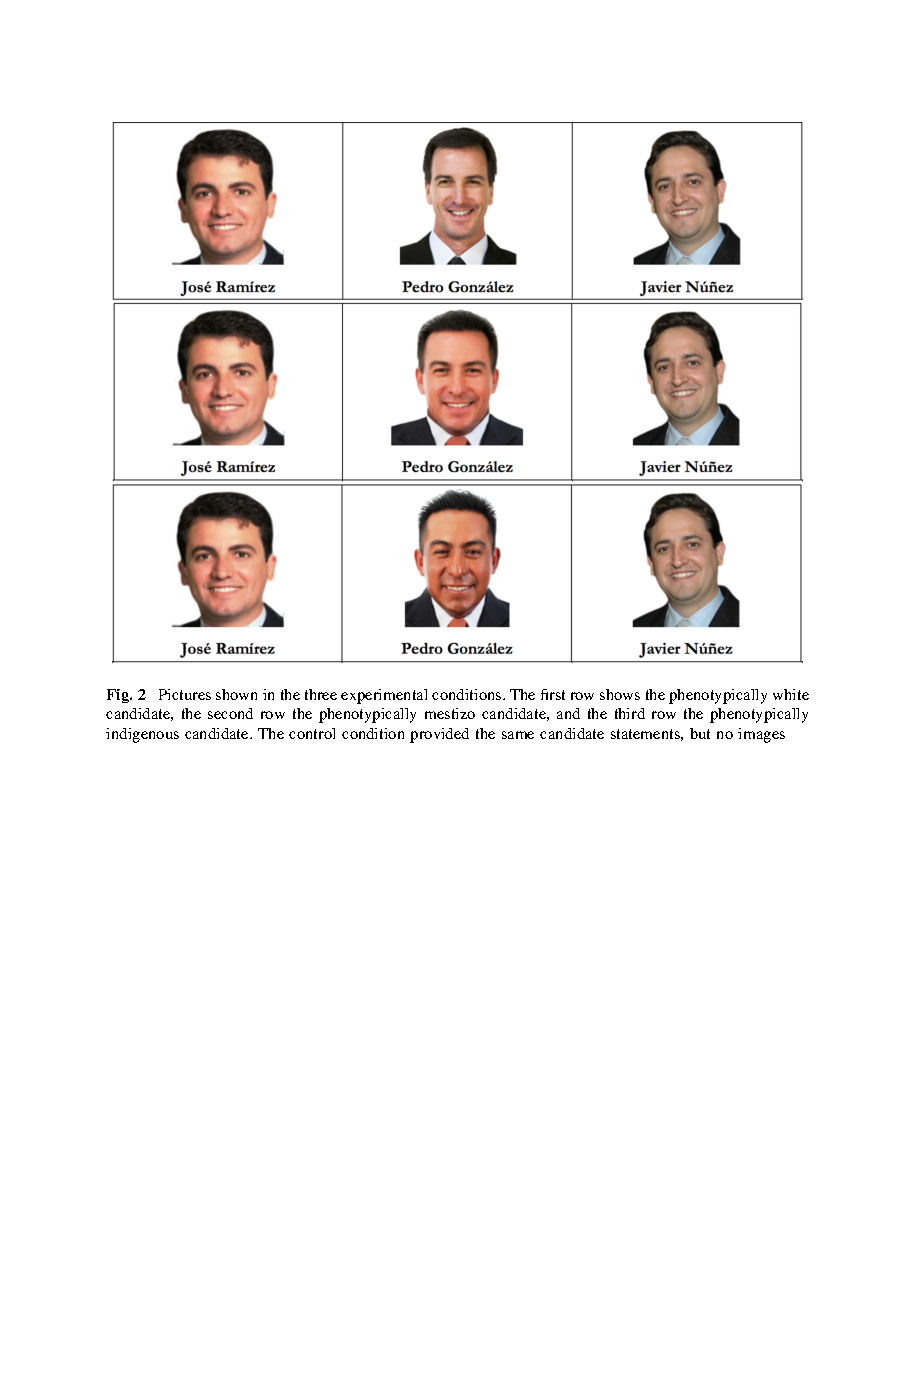
\includegraphics[width=0.8\linewidth]{./figs/survey-exp-aguilar-18} 

}

\end{figure}

Outcome: Candidate Choice (Aguiler et al 2018).
\end{frame}

\begin{frame}{Videos}
\protect\hypertarget{videos}{}
\begin{figure}

{\centering 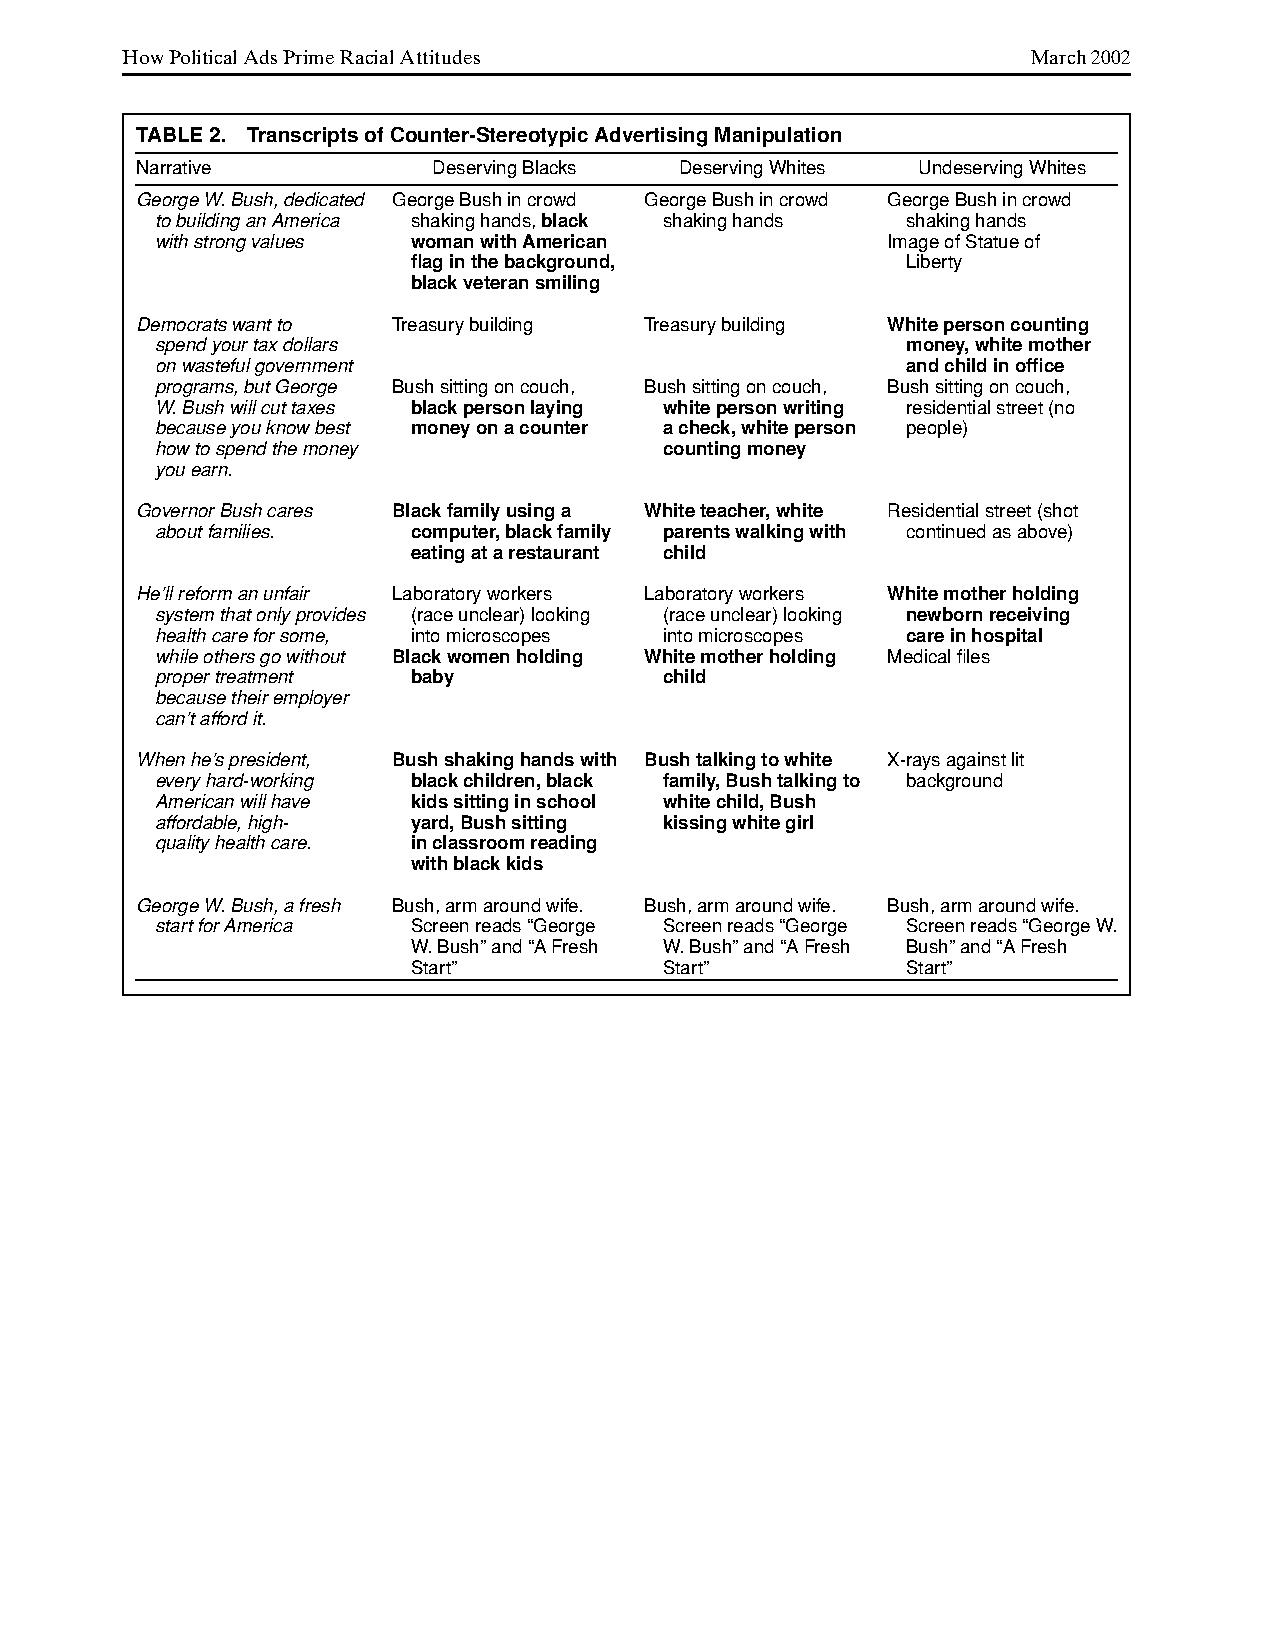
\includegraphics[width=0.65\linewidth]{./figs/survey-exp-valentino-2002} 

}

\end{figure}

Outcome: Candidate preference (Gore vs.~Bush).

(Valentino et al, 2002)
\end{frame}

\begin{frame}{Vignette}
\protect\hypertarget{vignette}{}
Effect of a set of information about corruption on support for
politicians:

\begin{quote}
Imagine a person named Gabriel (or Gabriela), who is a person like you,
living in a neighborhood like yours, but in a different city in Brazil.
The mayor of Gabriel's city is running for reelection in October. He is
a member of the PT {[}Partido dos Trabalhadores{]} (or PSDB {[}Partido
da Social Democracia Brasileira{]}). In Gabriel's city, it is well known
that the mayor never takes bribes (or frequently takes bribes) when
giving out government contracts. The mayor has completed few (or many;
or omit the entire sentence) public works projects during his term in
office. In this city, the election for mayor is expected to be very
close.
\end{quote}

(Winters and Weitz-Shapiro, 2013)
\end{frame}

\begin{frame}{Conjoint}
\protect\hypertarget{conjoint}{}
\begin{figure}

{\centering 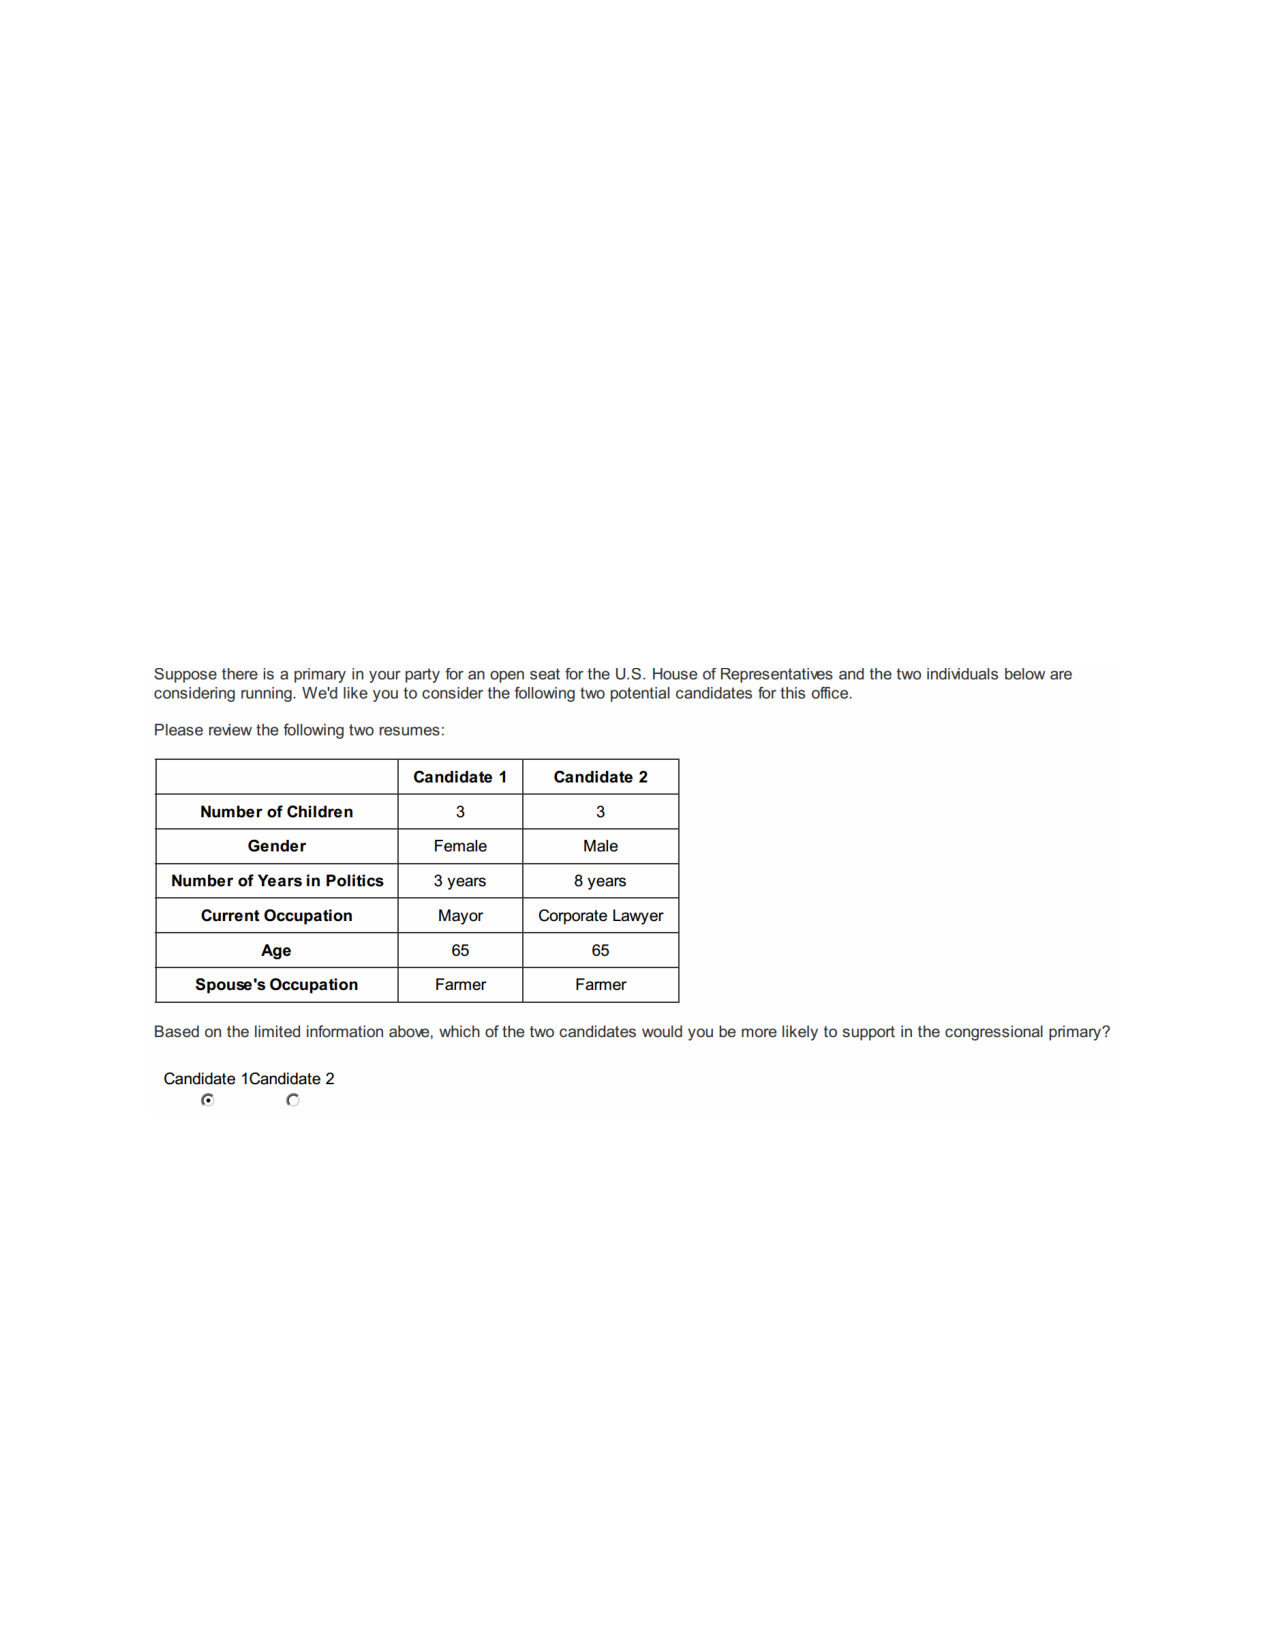
\includegraphics[width=0.8\linewidth]{./figs/survey-exp-teele-2018} 

}

\end{figure}

\begin{figure}

{\centering 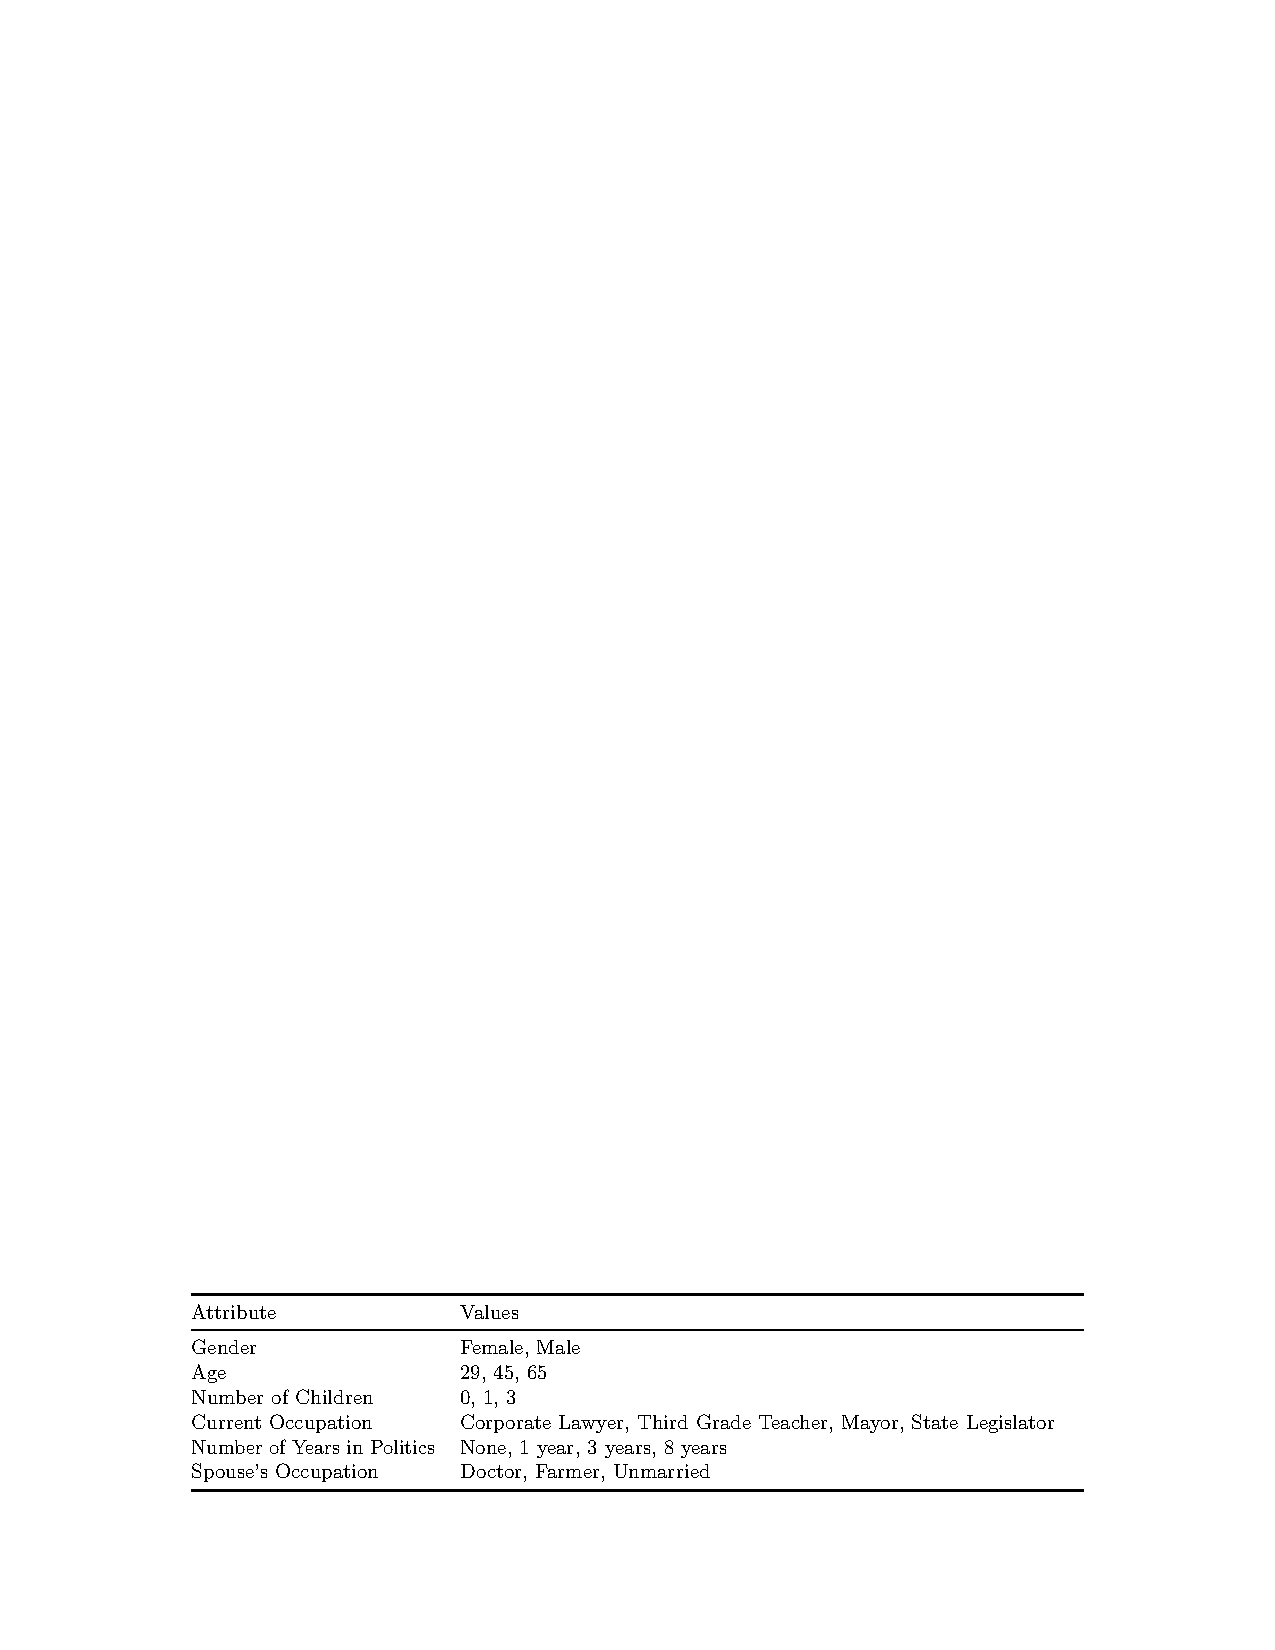
\includegraphics[width=0.8\linewidth]{./figs/survey-exp-teele-2018-conjoint-attributes} 

}

\end{figure}

(Teele et all 2018)
\end{frame}

\begin{frame}{Conjoint}
\protect\hypertarget{conjoint-1}{}
\begin{figure}

{\centering 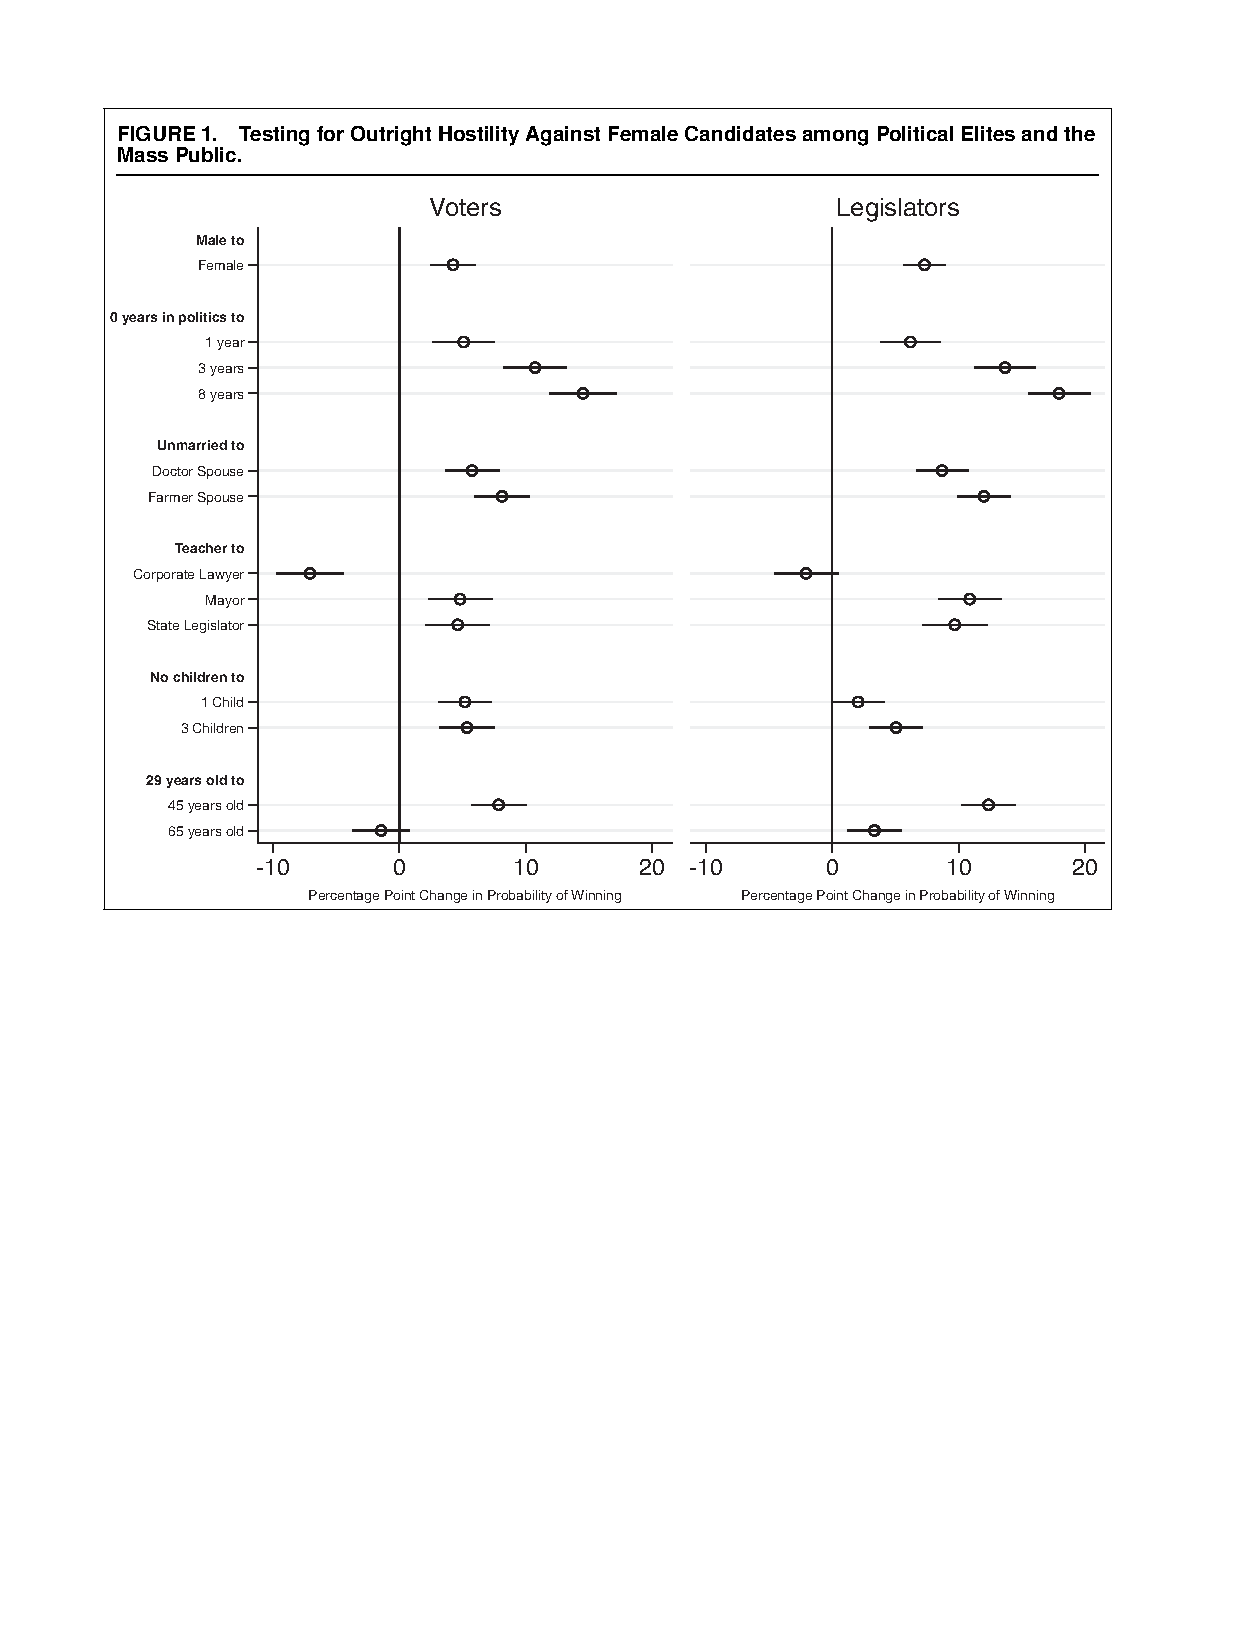
\includegraphics[width=0.8\linewidth]{./figs/survey-exp-teele-2018-results} 

}

\end{figure}

(Teele et all 2018)
\end{frame}

\begin{frame}{Conjoint Interpretation}
\protect\hypertarget{conjoint-interpretation}{}
People exposed to
\end{frame}

\hypertarget{examples-for-measurement}{%
\section{Examples for Measurement}\label{examples-for-measurement}}

\begin{frame}{Measurement of Concepts in General}
\protect\hypertarget{measurement-of-concepts-in-general}{}
Say we want to measure ``math ability''. We could

\begin{itemize}
\tightlist
\item
  watch people pay for coffee and make change (a behavioral measure
  capturing one aspect of math ability).
\item
  ask people on a survey ``What is 2+2?''
\item
  ask people on a survey ``Solve for \(x\) in \(y=x/2\).''
\item
  ask people \textbf{both} questions.
\end{itemize}

Often surveys allow multiple questions to measure concepts more cheaply
and quickly than watching behavior (Trading off measuring one concept
well versus other concepts less well.)

If the survey sample is representative, we learn about prevalence of a
given concept in a population.

For more on measurement in experiments (including field experiments) see
\href{https://egap.org/resource/10-things-to-know-about-measurement-in-experiments/}{10
Things to Know About Measurement in Experiments}
\end{frame}

\begin{frame}[shrink]{Measurement of Sensisitive Topics: Example of the
List Experiment}
\protect\hypertarget{measurement-of-sensisitive-topics-example-of-the-list-experiment}{}
Now I am going to read you three things that sometimes make people angry
or upset. After I read all three, just tell me HOW MANY of them upset
you. I don't want to know which ones, just HOW MANY.

\begin{enumerate}
[(1)]
\item
  the federal government increasing the tax on gasoline
\item
  professional athletes getting million-dollar contracts
\item
  large corporations polluting the environment
\end{enumerate}

\emph{(4) a black family moving in next door} (randomly assigned to half
of the respondents)

Baseline Condition: Only 3 items

Sensitive Item Condition: Add the ``black family'' item (4 items total)

Outcome: Did more people choose 4 items in the ``sensitive item''?

(Kuklinski 1997)

For more on measurement of sensitive topics in survey experiments see
\href{https://egap.org/resource/10-things-to-know-about-survey-experiments/}{10
Things to Know About Survey Experiments}.
\end{frame}

\hypertarget{general-considerations-in-interpreting-results-from-survey-experiments}{%
\section{General Considerations in Interpreting Results from Survey
Experiments}\label{general-considerations-in-interpreting-results-from-survey-experiments}}

\begin{frame}{Considerations in Interpreting the results of Survey
Experiments}
\protect\hypertarget{considerations-in-interpreting-the-results-of-survey-experiments}{}
Are the survey respondents ``pre-treated'' by the political, social,
informational context?

Example:

Treatment: The researcher in June of 2022 randomly assigns people to
learn that Russia has invaded Ukraine.

Outcome: Attitudes toward Russia.

Did the reseacher learn about the effect of information about invasions
on attitudes toward the invader? What if this experiment had been done
in 2013? Or 2015 (just after the invasion of Crimea)?
\end{frame}

\begin{frame}{Compliance and Non-Randomized Comparisons}
\protect\hypertarget{compliance-and-non-randomized-comparisons}{}
Did the respondent \textbf{understand} and/or \textbf{absorb} or
otherwise \textbf{attend to} the treatment (Manipulation checks;
Attention Checks).

For example, this Attention Check:

\begin{figure}

{\centering 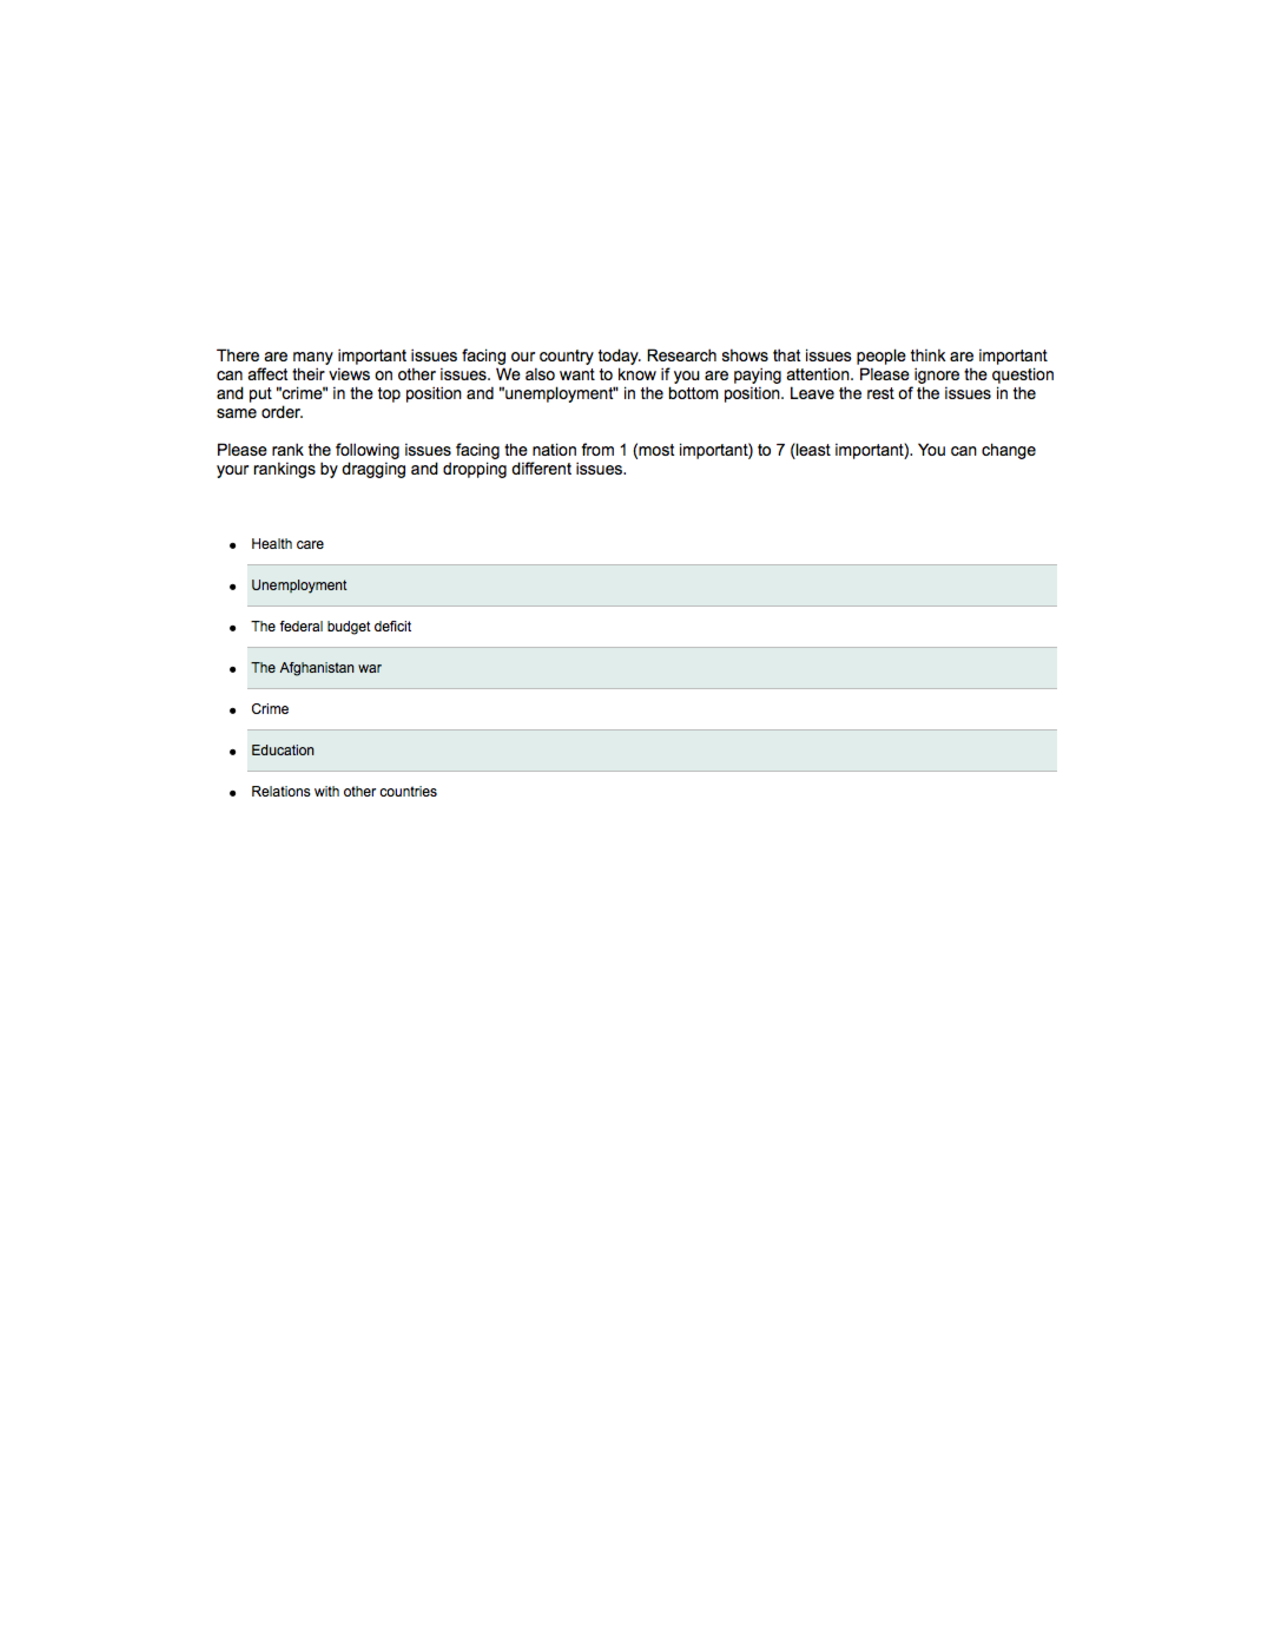
\includegraphics[width=0.7\linewidth]{./figs/survey-exp-berinsky_2019} 

}

\end{figure}

(Berinsky et al, 2019)
\end{frame}

\begin{frame}{Compliance and Non-Randomized Comparisons}
\protect\hypertarget{compliance-and-non-randomized-comparisons-1}{}
Did the respondent \textbf{understand} and/or \textbf{absorb} or
otherwise \textbf{attend to} the treatment (Manipulation checks;
Attention Checks).

For example a Manipulation Check done after the survey might say: ``Was
the name of the person in the vignette you just read (a) Maarten (b)
Gabriella (c) Jake or (d) Nahomi?''

\textbf{Questions:}

\begin{itemize}
\item
  What should you do if 25\% of your respondents fail the Manipulation
  Check?
\item
  Should your attention check come before or after randomization? What
  should you do with people who fail an attention check?
\end{itemize}
\end{frame}

\begin{frame}[fragile]{Moderation and Post-Treatment Bias}
\protect\hypertarget{moderation-and-post-treatment-bias}{}
If the theory implies a moderated relationship (high and low income
respondents should react differently to the randomized tax rate), is the
moderator asked \textbf{after} or \textbf{before} the treatment during
the survey?

If \textbf{after} could the treatment possibly affect the moderator?

You might mislead yourself if you calculated different effects by
subgroups where subgroup membership is caused by treatment. (If all
treated subjects report high income and all control subjects report low
income, then an analysis of treatment effects within subgroup is no
longer a randomized comparison --- and in this case would just return
\texttt{NA} values.)
\end{frame}

\begin{frame}{Lack of information equivalence and SUTVA Violations}
\protect\hypertarget{lack-of-information-equivalence-and-sutva-violations}{}
Not everyone understands the treatment the same way (Dafoe et al 2018):
(from Bowers 1998):

\begin{figure}

{\centering 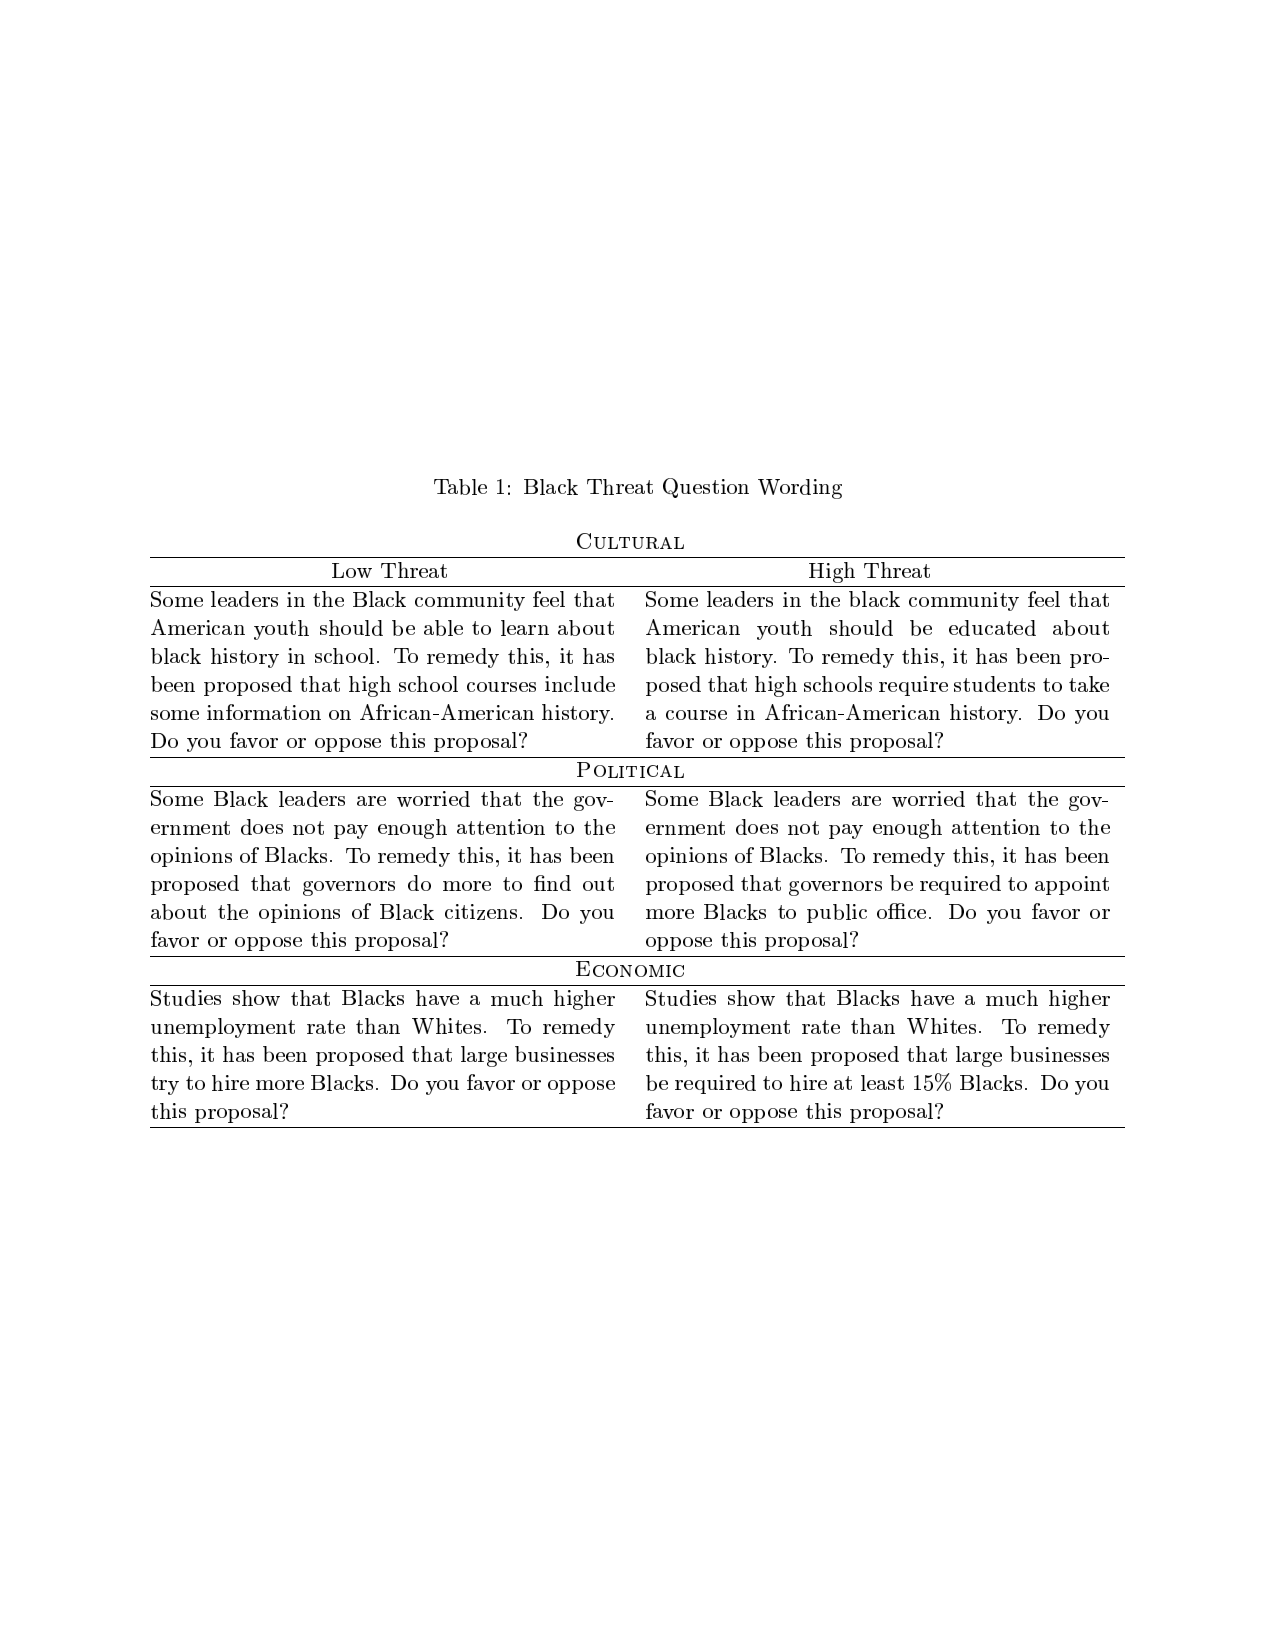
\includegraphics[width=0.8\linewidth]{./figs/survey-exp-bowers-1998-black-threat} 

}

\end{figure}
\end{frame}

\begin{frame}{Lack of information equivalence and SUTVA Violations}
\protect\hypertarget{lack-of-information-equivalence-and-sutva-violations-1}{}
Not everyone understands the treatment the same way (Dafoe et al 2018):
(from Bowers 1998):

\begin{figure}

{\centering 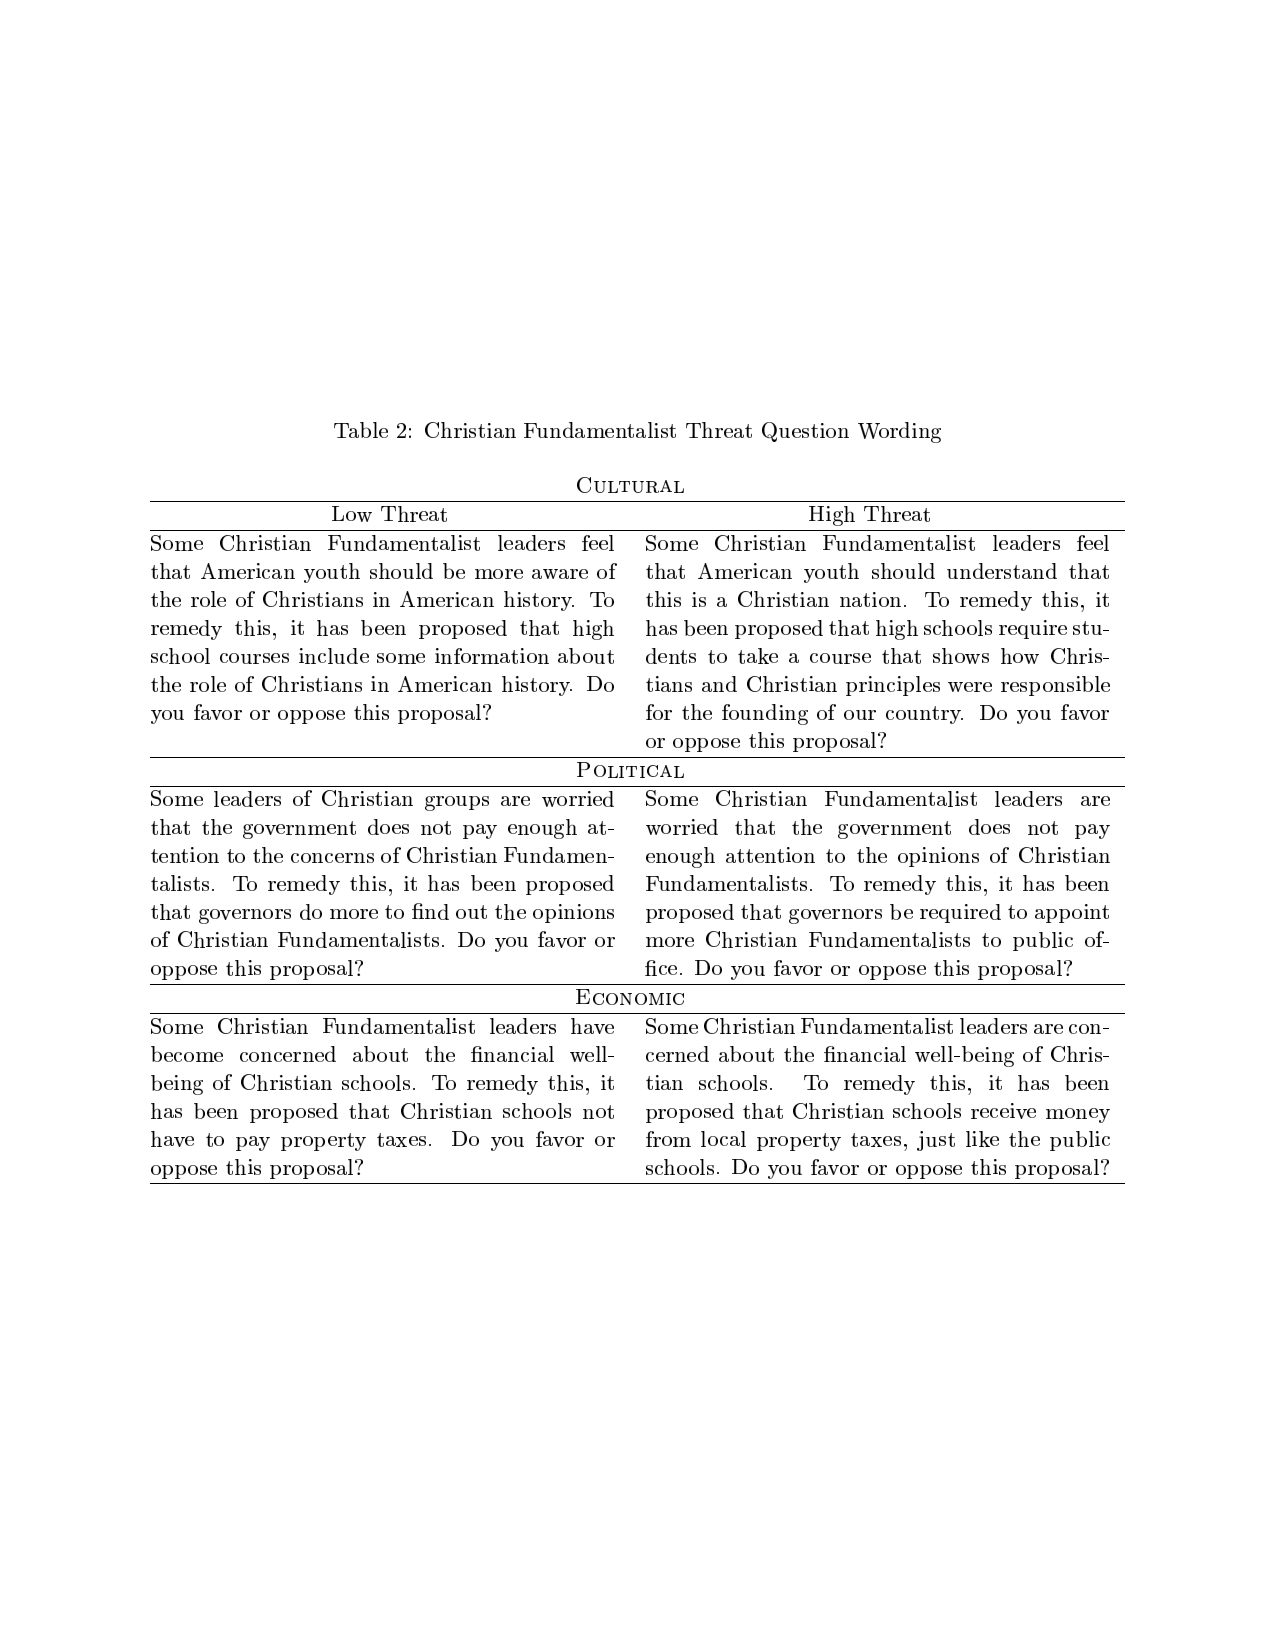
\includegraphics[width=0.8\linewidth]{./figs/survey-exp-bowers-1998-christian-threat} 

}

\end{figure}
\end{frame}

\begin{frame}[allowframebreaks]{Other issues of interpretation}
\protect\hypertarget{other-issues-of-interpretation}{}
\begin{itemize}
\tightlist
\item
  Do interpretations of the treatment depend on other questions asked
  previously? (Not a problem of bias, but of interpretation).
\item
  What are alternative arguments about the \textbf{meaning} of the
  treated-to-control comparison? (Does hearing ``Gabriel'' or
  ``Gabriela'' raise certain considerations in respondents' minds that
  would change if they were asked about ``Jens Olaf'' or ``Shuyuan''?)
\item
  Remember that a treatment effect is a comparison of two groups --- in
  survey experiments the ``control'' condition tends not to be a status
  quo condition
\item
  Does it matter than the effect of exposure to a survey treatment might
  go away within minutes or seconds? Does it matter (and how and when)
  that the outcome of a survey experiment is often measured within
  seconds or minutes of the treatment? Can a short duration effect teach
  us about theory?
\item
  Many online experimental pools are not representative samples. When
  might this matter? When might this not matter
\item
  How to interpret experimental comparisons with no natural control
  group? Should Winters and Weitz-Shapiro have had a pure control
  condition? Or could the difference in \emph{time} or \emph{effort}
  between a survey requiring someone to read a vignette and a survey
  that skips the vignette confuse interpretation of the findings?
\end{itemize}
\end{frame}

\begin{frame}{Realism and Learning about Theory}
\protect\hypertarget{realism-and-learning-about-theory}{}
What do we learn from survey respondents' short term reactions to
hypothetical choices and situations?

\begin{quote}
``In your opinion, what is the likelihood that Gabriel(a) will vote for
this mayor in the next election: very likely, somewhat likely, unlikely,
not at all likely?''
\end{quote}

Winters and Weitz-Shapiro(2013) and Boas et al (2018) found negative
effects of corruption information in survey experiments in Brasil. Boas
et al (2018) found no effects of providing corruption information on
voting in a field experiment.

\medskip

\textbf{Question:} What is the role of survey experiments in a research
program? How can survey experiments contribute? .
\end{frame}

\hypertarget{references}{%
\section*{References}\label{references}}
\addcontentsline{toc}{section}{References}

\begin{frame}{References}
\hypertarget{refs}{}
\begin{CSLReferences}{1}{0}
\leavevmode\vadjust pre{\hypertarget{ref-mutz2011population}{}}%
Mutz, Diana C. 2011. \emph{Population-Based Survey Experiments}.
Princeton University Press.

\end{CSLReferences}
\end{frame}

\end{document}
